\documentclass{beamer}
\usetheme{Freiburg}
\usepackage{mystyle2}
%\beamersetuncovermixins{\opaqueness<1>{25}}{\opaqueness<2->{15}}
\begin{document}

\title[]{The Determination of Gradients on Enemy-Held Beaches\\ W.W. Williams, 1946}   %Der Titel des Vortrages
\subtitle[]{or\\\emph{How to Measure a Beach Without Being Shot}}
\author{Kieran Newman} %Der Autor bzw. der Redner
\date{5th November 2015} % also heute 

\frame{\titlepage}

\section{Motivation}

\begin{frame}
\frametitle{Motivation}
\begin{itemize}
\item Autumn, 1941 - Planning for Allied invasion of France
\end{itemize}
\begin{figure}
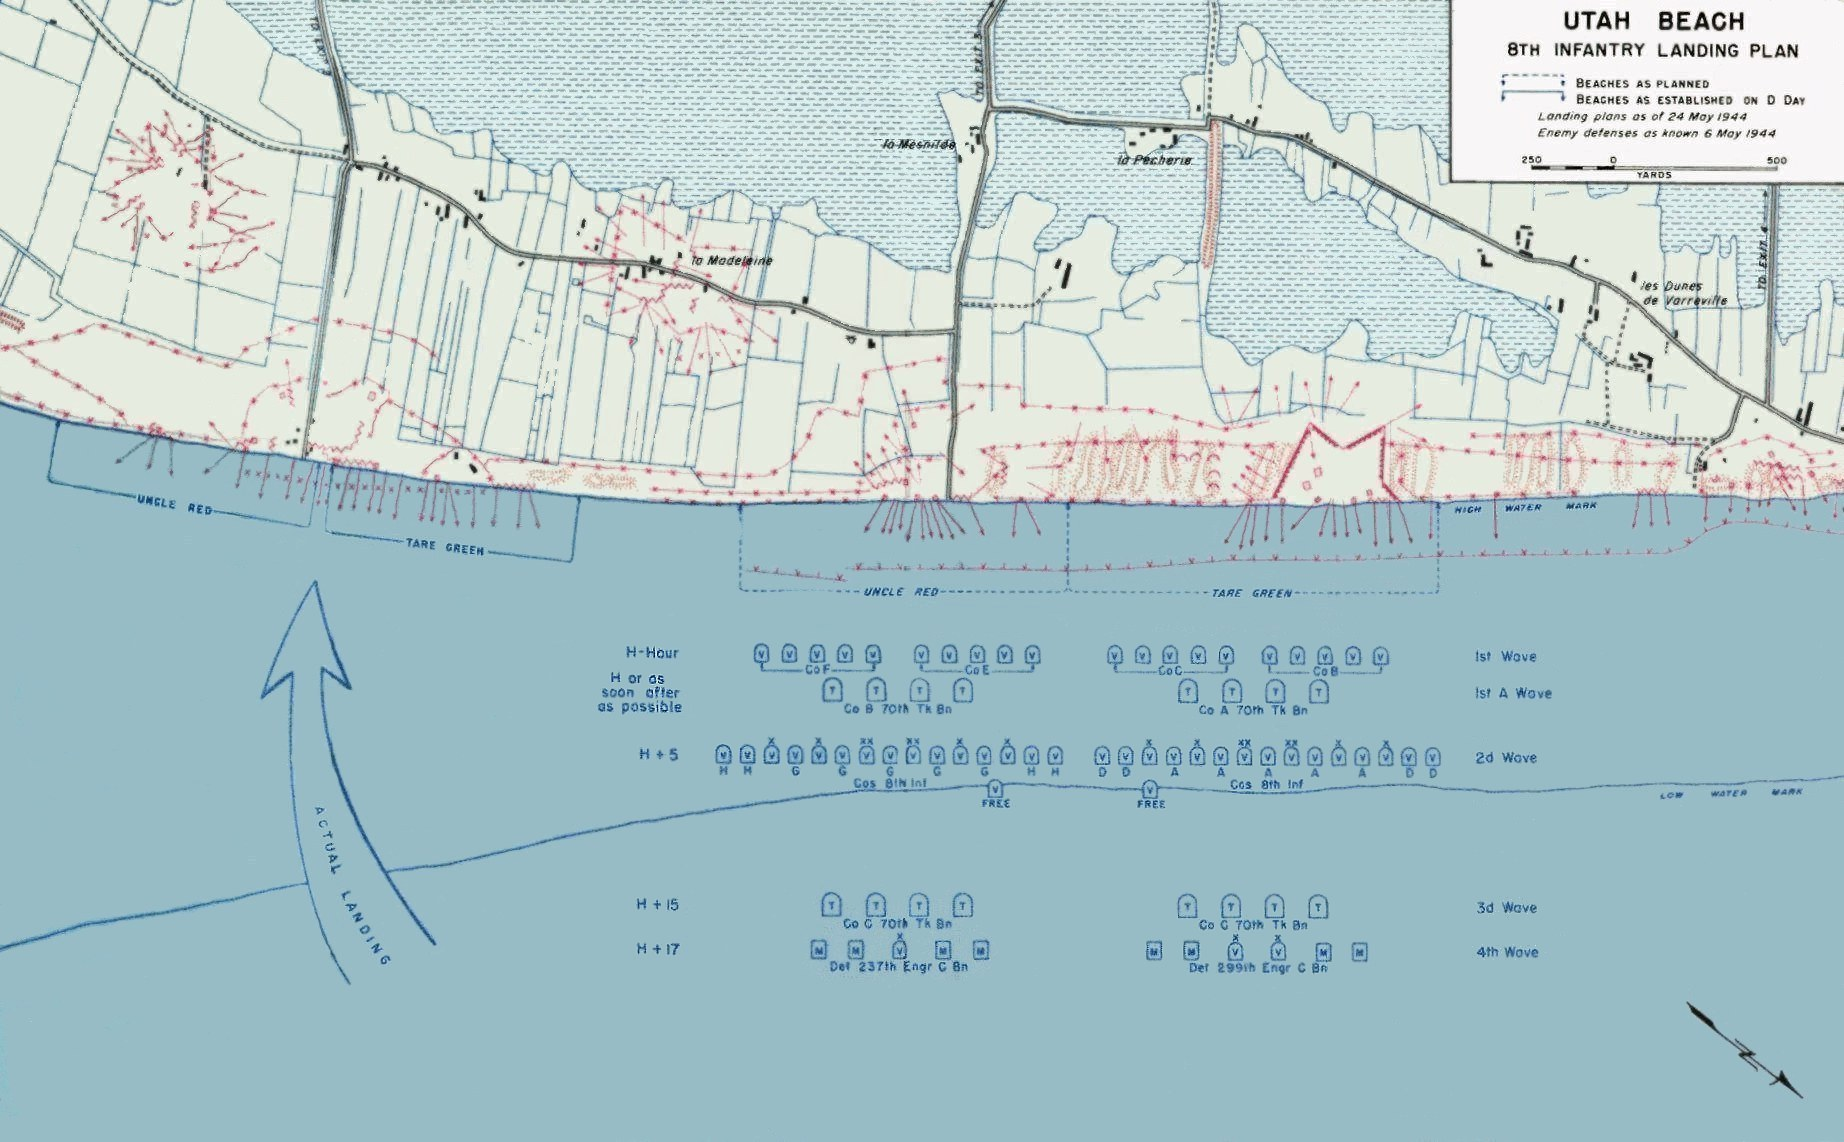
\includegraphics[width=\linewidth]{Utah_beach_landingplan}
\caption{Landing plan for Utah Beach, 1944. From \emph{Utah Beach to Cherbourg (6 June-27 June 1944). Washington, Historical Division, Department of the Army, 1947.}}
\end{figure}
\end{frame}

\section{Details of the Method}

\section{Results and Validation}

\section{Further Developments and Modern Methods}


\begin{frame}
\centering
\vspace{0.51in}
Thankyou for your time.


Please feel free to ask any questions.
\end{frame}
\bibliographystyle{dcu}
\bibliography{kwnrefs}
\end{document}
